\section{\label{II-B-2}Des \textit{Knowledge Organization Systems} (KOS) à \ac{skos}: vers l'interopérabilité syntaxique}
\titreEntete{Vers l'interopérabilité syntaxique}

%intro
Les ontologies ressemblent fortement aux \textit{thesauri} et autres vocabulaires contrôlés --- les \ac{kos} --- à cause du contrôle de la graphie, des termes retenus ou rejetés, et de l'établissement de relations entre les termes. Cependant, une ontologie n'est pas nécessairement un thésaurus, alors qu'un thésaurus est une ontologie. Bien que la distinction entre les deux soit mince, elle est essentielle en raison du formalisme qui compose les ontologies.\\

L'interopérabilité sémantique permise par les ontologies bâtit de l'interconnexion entre les jeux de données, rend possible l'échange et la publication de données nativement différentes sur le Web de données. La conversion par les institutions patrimoniales d'une partie ou de l'ensemble de leurs vocabulaires en ontologies a été permise par l'ontologie \ac{skos}.

\subsection{\label{II-B-2-a}Distinguer les systèmes d'organisation de la connaissance des ontologies}
\titreEntete{Distinguer les KOS des ontologies}

Les \ac{kos} sont des référentiels contrôlés de vedettes et de termes qui ne sont valables que pour un domaine d'activité et de la connaissance. Ils sont souvent organisés par des relations terminologiques et sémantiques qui les font se confondre avec les ontologies en raison de leur formalisation\footcite[p.48]{dalbin_approches_2011}. Plus encore, sur le Web de données, les \ac{kos} ne jouent pas de rôle, ils n'apportent pas de structure, mais complètent des référentiels ou des jeux de données déjà existants. Les \ac{kos} n'offrent qu'une succession de termes destinés à remplir des champs descriptifs, alors que les ontologies dirigent directement les données et leur structure.\\

Les ontologies permettent de dépasser certaines limites des \ac{kos} relevées dans la \reference{controler}\footcite{isaac_les_2012}:
\begin{itemize}
	\item les \textit{thesauri} et autres vocabulaires sont destinés d'abord à un utilisateur humain qui peut facilement comprendre la structure du vocabulaire\footnote{C'est le cas de la visualisation graphique du thésaurus des noms communs de l'\ac{ina}. Voir \reference{annexe_thesaurus} (\reference{thesaurus_cadreur}).}; les ontologies visent quant à elles à d'abord être comprises par une machine et le Web sémantique;
	\item les \ac{kos} induisent souvent des relations diverses et variables, notamment dans le cas de relations génériques--spécifiques
\end{itemize}
\medskip
Les limites identifiées sont dues principalement aux relations des termes des \ac{kos}: ces vocabulaires ne sont pas sémantiques, seulement hiérarchiques dans le but de classer et d'aider l'humain dans la compréhension du contexte du terme. L'apport des ontologies est l'ajout de sens aux termes grâce aux relations qu'ils entretiennent entre eux.


\subsection{\label{II-B-2-b}\ac{skos}: exposer les systèmes d'organisation de la connaissance sur le Web de données}
\titreEntete{SKOS: exposer les KOS sur le Web de données}

Dans le but de permettre aux institutions d'établir des liens entre leurs référentiels et leurs données, \ac{skos} a été créé. \ac{skos} est \og une ontologie qui se veut simple et compatible avec une majorité d’approches d’organisation des connaissances existantes (thésaurus, classifications\dots)\fg{}\footcite[p.8]{isaac_les_2012}. Elle permet de représenter presque tous les types de vocabulaires en concepts liés. \ac{skos} n'est pas un référentiel, seulement un moyen de faciliter l'interconnexion entre les données, leur échange, et de créer de nouveaux usages jusqu'alors impossibles.\\

Pour cela, \ac{skos}, vocabulaire \ac{rdf}, reprend les propriétés des vocabulaires contrôlés, notamment du thésaurus. En effet, il est possible d'indiquer des termes préférentiels, alternatifs, traduits, variants, \dots~;de plus, des notes peuvent être introduites; enfin, des liens --- génériques et hiérarchiques, associatifs, \dots~ sont créés entre les différents concepts\footnote{Voir \reference{skos_modelisation}.}. \ac{skos} a le rôle de l'essieu dans le modèle de l'interopérabilité de la roue et de l'essieu. Elle offre un petit nombre de concepts servant à la description et à la transcription d'un thésaurus dans un langage compréhensible par une machine. Ainsi, \ac{skos} est une ontologie de domaine: elle hérite d'autres ontologies comme DC Terms ou \ac{rdfs}, et sert d'ontologie de haut niveau pour des ontologies de plus bas niveau\footnote{La consultation de \url{https://lov.linkeddata.es/dataset/lov/vocabs/frbr} permet de constater ce rôle pivot de \ac{skos} pour les autres ontologies, ainsi que sa dépendance à d'autres ontologies.}.\\

\begin{figure}[!h]
	\centering
	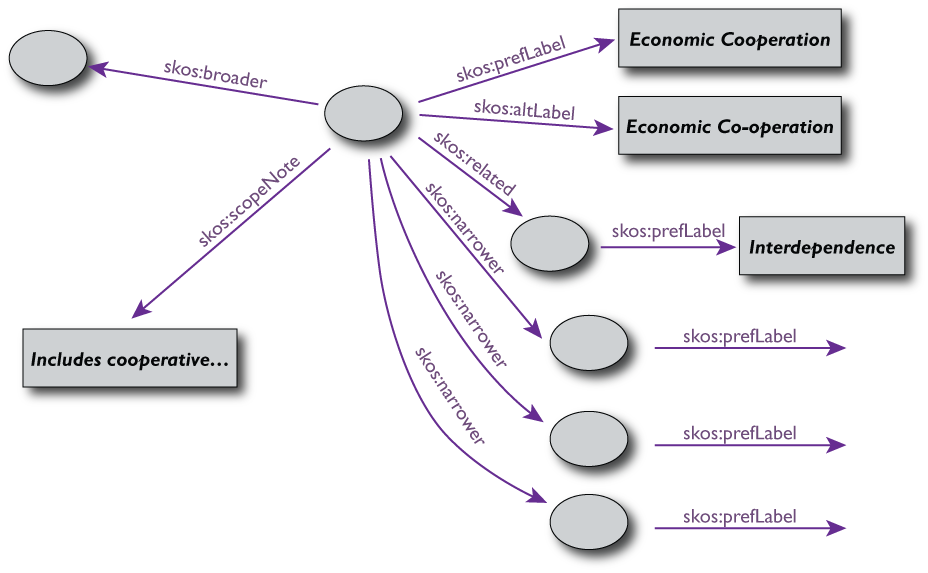
\includegraphics[width=13cm]{images/SKOS_simpleThesaurus.png}
	\caption[Modélisation simplifiée de \ac{skos}]{Modélisation simplifiée de \ac{skos} [Source: \href{https://www.w3.org/Consortium/Offices/Presentations/RDFTutorial/figures/SKOS_simpleThesaurus.png}{www.w3.org}]}
	\label{skos_modelisation}
\end{figure}
\medskip

Enfin, des propriétés de \ac{skos} permettent de créer du lien entre des concepts provenant de différentes sources: ce sont les propriétés d'équivalence ou de similitude <skos:broader>, <skos:exactMatch> ou <skos:closeMatch>. Ces propriétés permettent le rapprochement de plusieurs concepts: le \ac{lcsh}\footnote{Voir \reference{lcsh_liens}.} peut ainsi utiliser \ac{skos} pour créer des fiches de liens. De même, la Bibliothèque nationale de France (BnF) contient des références à l'ontologie Dewey qui lui permet ainsi d'obtenir des relations d'équivalence avec ses données. Alors, l'emploi de \ac{skos} nécessite des URIs de manière à créer des triplets \ac{rdf}.\\

Avec \ac{skos}, l'interopérabilité sémantique est désormais possible entre les institutions sur le Web de données. Cette ontologie \ac{rdf} permet de rapprocher des jeux de données et des référentiels jusqu'alors séparés et pourtant similaires. Le vocabulaire offert pour décrire les \textit{thesauri} et ensuite les partager dans le Web sémantique permet de nombreuses applications en institutions, et facilite ainsi les opérations d'indexation ou de recherche.

%conclu
\bigskip
\bigskip
Cependant, les vocabulaires des institutions n'étant pas nativement liés entre eux, il reste difficile de les aligner, et par conséquent de passer d'un \ac{kos} à une modélisation \ac{skos}, notamment pour les relations partie--tout. \nP{Sylvie}{Dalbin} prend en exemple\footcite{dalbin_approches_2011} ce type de relation qui peut être exprimé dans le Web sémantique par trois types de relations: hiérarchique, instance--classe, ou bien sous-classe--classe. Ces incertitudes rendent le processus d'ontologisation complexe, qui l'est d'autant plus quand les termes sont dans des langues différentes.\\

Les ontologies apparaissent comme un référentiel essentiel dans le Web de données, plus encore que les autorités qui sont devenues des données; elles ont permis l'apparition d'un Web sémantique. Seulement, la problématique de l'alignement de référentiels entre eux sur le Web de données est toujours présente et ne sera jamais totalement résolue.